\documentclass{article}
\usepackage{graphicx} % Required for inserting images

\title{IS_arhitektura}
\author{stevandragovic.10 }
\date{December 2023}

\begin{document}

\section{Arhitektura sistema}

U ovom poglavlju cemo opisati arhitekturu našeg sistema. Pri odabiru arhitekture cilj je bio da ima dobru podelu odgovornosti, da bude jednostavna za održavanje, da bude bezbedna, stabilna i jednostavna za razumevanje. Tip arhitekture je klijent-server, gde se komunikacija vrši uz pomoć HTTP zahteva, gde klijent ima aktivnu ulogu, ulogu pošiljaoca zahteva, dok server ima pasivnu ulogu, ulogu primaoca zahteva od klijenta. U tom tipu komunikacije, broj klijentskih računara odgovara broju aktera našeg sistema, ukupno pet, dok je broj serverskih računara 1.
\newline
\newline
\newline
Kod arhitekture servera, odabrana je slojevita arhitektura, koja ima 5 slojeva:
\begin{enumerate}
    \item Prezentacioni sloj
    \item Infrastrukturni sloj
    \item Sloj slučajeva upotrebe 
    \item Sloj servisa
    \item Sloj entiteta
\end{enumerate}
Kako su slojevi organizovani, može se videti na sledećoj slici 

\begin{center}
    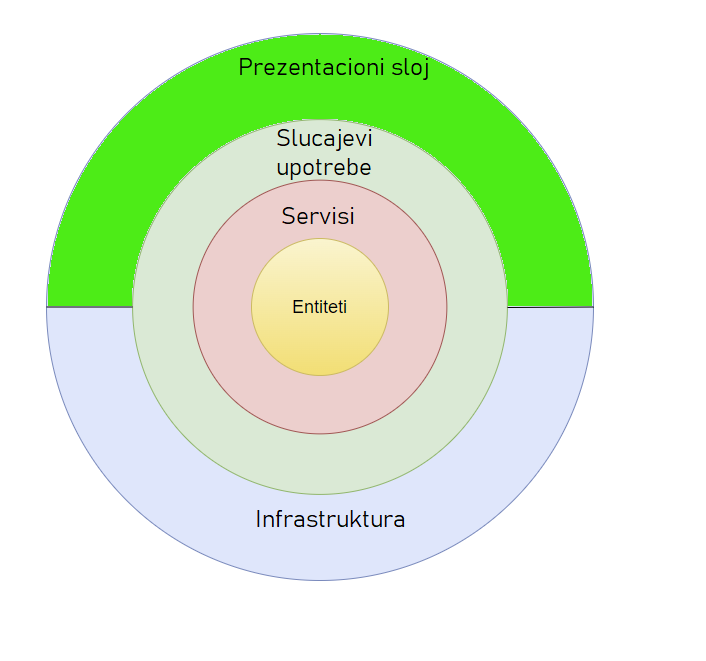
\includegraphics[scale=0.5]{arhitekturaSistema.png}
\end{center}

Slojevi su organizovani tako da su unutrašnjih slojevi nezavisni od spoljašnjih slojeva, svaki od njih ima jedinstvenu odgovornost čime pošujemo princip "Jedinstvena odgovornost" u OOP i što omogućava jednostavniji razvoj sistema. Ovakav izbor slojeva omogućava visoku granuliranost, i to se postiže principom "Inverzija zavisnosti". Ovakva organizacija arhitekture odgovara obrascu "Čista arhitektura".
\newline
\newline
Opis slojeva:
\newline
\begin{enumerate}
    \item Prezentacioni sloj - predstavlja ulaznu tačku našeg sistema. On prihvata podatke od klijenta, i šalje ih dalje sloju slučajeva upotrebe.
    \item Sloj slučajeva upotrebe - sadrži sve slučejeve upotrebe opisane za naš sistem. Ovim želimo da naša arhitektura bude orijentisana prema opisanim slučajevima upotrebe, tako da budućim čitaocima opisa našeg sistema bude jasno šta naš sistem zapravo radi. 
    \item Sloj entiteta - predstavlja centralni deo biznis logike našeg sistema. Ne zavise od spoljnih detalja sistema, kao što su drajveri, radni okviri i ostalo.
    \item Sloj servisa - pored sloja entiteta, sadrži i interfejs za korišćenje baze podataka
    \item Infrastrukturni sloj - Zavisi od sloja servisa, gde se dešava implementacija interfejsa za korišćenje baze podataka.
\end{enumerate}



Zavisnost slojeva prikazana je na sledećoj slici.


\begin{center}
    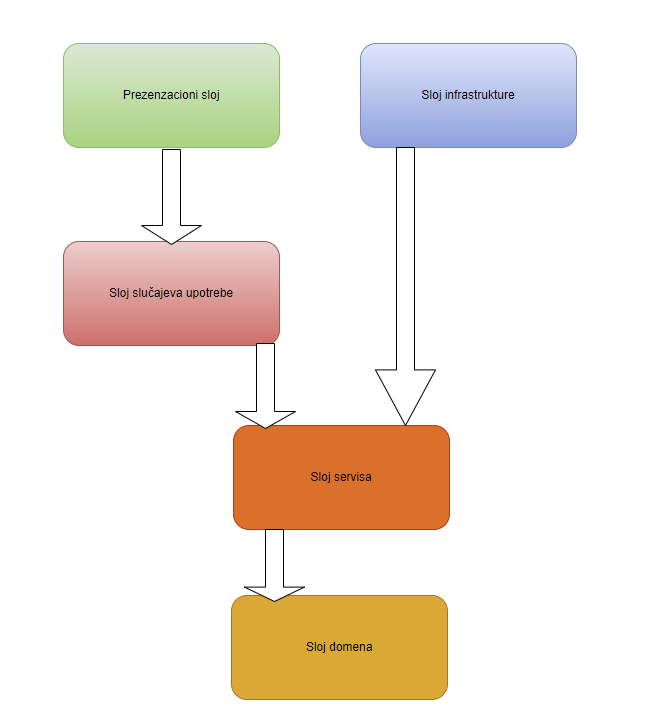
\includegraphics[scale=0.5]{zavisnostSlojeva.png}
\end{center}

\begin{center}
  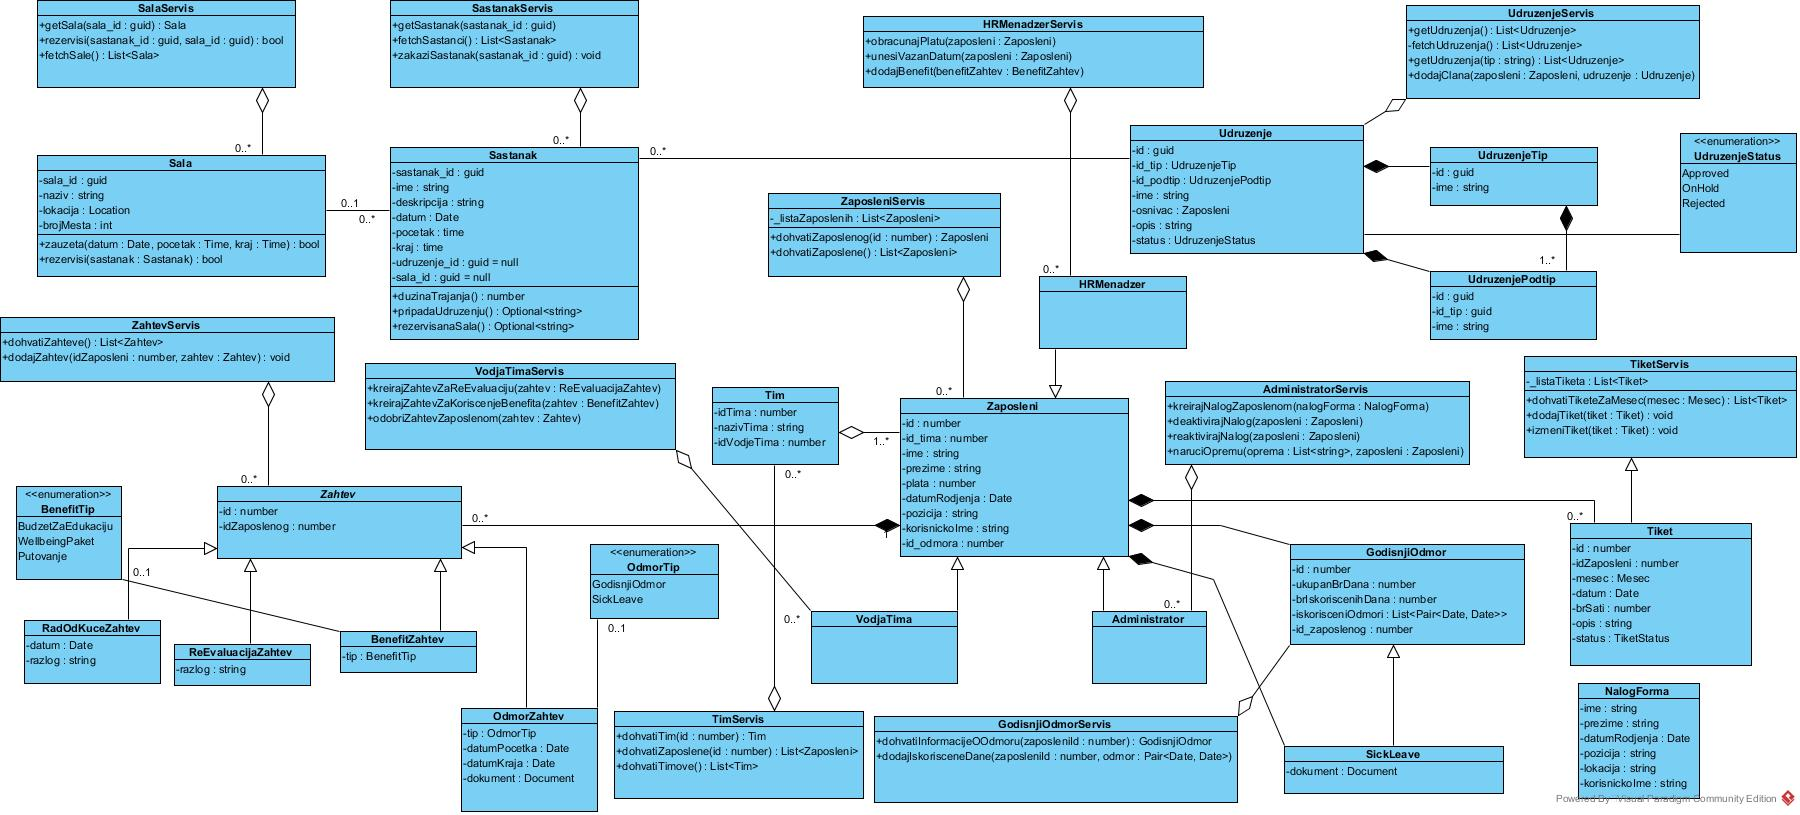
\includegraphics[scale=0.3, angle=90]{EvidencijaZaposlenihKlasniDijagram.jpg}
\end{center}

\end{document}
